%%%%%%%%%%%%%%%%%%%%%%%%%%%%%%%%%%%%%%%%%%%%%%%%%%%%%%%%%%%%%%%%%%%%%%%%%%%%%%%%
%2345678901234567890123456789012345678901234567890123456789012345678901234567890
%        1         2         3         4         5         6         7         8

\documentclass[letterpaper, 10 pt, conference]{ieeeconf}  % Comment this line out if you need a4paper

%\documentclass[a4paper, 10pt, conference]{ieeeconf}      % Use this line for a4 paper

\IEEEoverridecommandlockouts                              % This command is only needed if 
                                                          % you want to use the \thanks command

\overrideIEEEmargins                                      % Needed to meet printer requirements.

%In case you encounter the following error:
%Error 1010 The PDF file may be corrupt (unable to open PDF file) OR
%Error 1000 An error occurred while parsing a contents stream. Unable to analyze the PDF file.
%This is a known problem with pdfLaTeX conversion filter. The file cannot be opened with acrobat reader
%Please use one of the alternatives below to circumvent this error by uncommenting one or the other
%\pdfobjcompresslevel=0
%\pdfminorversion=4

% See the \addtolength command later in the file to balance the column lengths
% on the last page of the document

% The following packages can be found on http:\\www.ctan.org
\usepackage{graphicx} % for pdf, bitmapped graphics files
%\usepackage{epsfig} % for postscript graphics files
%\usepackage{mathptmx} % assumes new font selection scheme installed
%\usepackage{times} % assumes new font selection scheme installed
%\usepackage{amsmath} % assumes amsmath package installed
%\usepackage{amssymb}  % assumes amsmath package installed
\usepackage{amsfonts}

\title{\LARGE \bf
Improving Vehicle Localization in Urban Canyons using SLAM and Semantic Point Cloud Registration
}

\author{Alexander Jaeckel, Ryan Jones, Timothy Potts, and Rakkappan Baskaran\\% <-this % stops a space
Email: ajaeckel@umich.edu, ryajones@umich.edu, tpotts@umich.edu, rbaskara@umich.edu
}

\begin{document}

\maketitle
\thispagestyle{empty}
\pagestyle{empty}


%%%%%%%%%%%%%%%%%%%%%%%%%%%%%%%%%%%%%%%%%%%%%%%%%%%%%%%%%%%%%%%%%%%%%%%%%%%%%%%%
\begin{abstract}

Abstract placeholder

\end{abstract}


%%%%%%%%%%%%%%%%%%%%%%%%%%%%%%%%%%%%%%%%%%%%%%%%%%%%%%%%%%%%%%%%%%%%%%%%%%%%%%%%
\section{INTRODUCTION}

Many autonomous and semi-autonomous systems are not robust enough to operate in all areas of the world. Low quality of lane lines, curves that are too tight, and other environmental noise factors can cause the performance of these systems to decrease to unacceptable levels. A common strategy to deal with these noise factors is to restrict the degree of autonomous support offered in an area that has high environmental noise factors. This practice is called geo-fencing. In systems that employee geo-fencing it is critical that the system is able to accurately localize to a known map. If the vehicle incorrectly localizes, then a higher degree of autonomous support may be offered than is safe for that area. In many areas GPS is sufficient to determine the correct location of the vehicle. In some areas however this is more challenging. One area that offers a particular challenge is densely populated urban cities.  In these areas GPS performance suffers due to the presence of tall buildings which create an effective urban canyon and induce multi-path effects in the GPS. When GPS becomes unreliable, we need another method for determining the current location of the vehicle.

\section{METHODS}

\subsection{Vehicle Input Data Processing}

Placeholder

\subsection{Map Data Processing}

Map Data Processing Placeholder

\subsection{Simultaneous Localization and Mapping}

\begin{figure}[thpb]
  \centering
  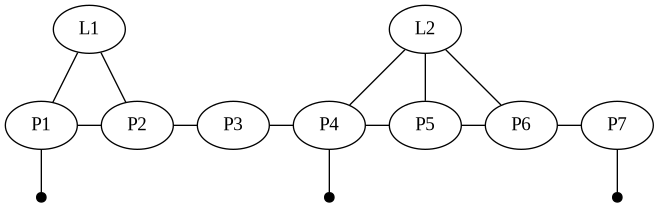
\includegraphics[width=\linewidth]{factor_graph.png}
  \caption{Example factor graph}
  \label{fig:factorgraph}
\end{figure}

In order to generate an initial trajectory estimate and local map of observed landmarks, we utilize a factor graph based SLAM method.
The variables in our factor graph consist of vehicle poses $X_t \in \mathrm{SE}(2)$ and landmark positions $L_n \in \mathbb{R}^2$.
Our vehicle data provides longitudinal velocity and yaw rate which can be combined into odometry factors $u_t \in \mathfrak{se}(2)$ between poses $X_t$ and $X_{t+1}$.
The GPS measurements $z_t \in \mathbb{R}^2$ are used as prior factors on the translational component of the current vehicle pose $X_t$ at the time that the measurement is obtained. Due to the difference in sampling rate of odometry and GPS data, not all poses will have an associated prior factor.
Each landmark observation consists of a landmark identifier $n$ and a distance to the landmark $v_i \in \mathbb{R}^2$ relative to the vehicle frame which is added as a factor between the pose $X_t$ at the time the measurement is obtained and the landmark location $L_n$.
An example simplified factor graph is shown in Figure \ref{fig:factorgraph}.

Variables and factors are added to the graph iteratively as new measurements become available.
To solve the factor graph we make use of the ISAM2 algorithm \cite{ref:isam} which internally converts the factor graph into a Bayes tree before optimizing. This approach allows for fast updates to variable estimates when adding new factors to the graph without the need for periodic batch relinearization or reordering.
Our final local map is the set of points of the best estimates of $L_n$ along with their semantic classes.

\subsection{Semantic Point Cloud Registration}
The odometry information used in the SLAM algorithm accumulates error over time. Without proper handling, this can cause the estimated trajectory to diverge from the true trajectory. The routine GPS signals received by the vehicle help to correct this (often they can give an acceptable level of localization by themselves), but these are also prone to error in certain circumstance, as discussed. This problem was alleviated by using a Semantic Iterative Closet Point (SICP) auces a transformation from the estimated, locally observed landmark locations to the known, global locations. This transformation can then be applied to the estimated vehicle trajectory to improve the accuracy of the estimate. 

The matching of the local map to the global map uses a variation of the ICP algorithm shown in the lecture slides (INSERT LECTURE REFERENCE HERE) that has been modified to include the semantic labelling of the vehicle input sign data. The code itself is built upon the gicp\_SE3 code written by Manni Ghaffari Jadidi [INSERT REFERENCE TO CODE HERE]. This code was modified to include semantic labeling in the nearest neighbor search and set the covariance normal to each point to the identity, removes the functionality of looking at distributions around points near each other. Pseudo-code for the algorithm is shows in FIGURE.lgorithm to match the local map of landmarks, produced during the SLAM step, to a known global map of landmarks. Matching these landmarks prod

The local and global landmark maps are used as the source and target point clouds, respectively. The initial transformation is estimated by using the previous GPS measurements. These most likely are not completely accurate but should be good enough for an initial estimate. For each landmark in the local map, we find the nearest neighbor [INSERT REFERENCE HERE FOR NEAREST NEIGHBOR ALGORITHM] of the same label in the global map. If a nearest neighbor of the same label cannot be found, or if it is further away than is allowable (tunable parameter), it is ignored for this iteration. Once a correlation between landmarks in the local map and target map have been found, a linear least squares problem is solved, which will produce a transformation in SE3. This transformation is then applied to the local landmark map, and the process is repeated until convergence or the maximum number of iterations (tunable parameter) is reached. If the algorithm does not converge, or if it does converge, but the average distance between correlated landmarks in the transformed local map and the global map is too high, then it will be ignored. Otherwise, the transformation is applied to the estimated trajectory to correct for the odometry and GPS drift.

The SICP algorithm needs a relatively large number of observed landmarks in the local map in order to accurately perform the semantic map registration, or else there is a risk of the algorithm not converging or converging to the wrong transformation. Since the maps we are using include 3 dimensions, we will need at least six different landmarks, but it is preferable to have more than that. It takes time for the local landmark map to be created as the vehicle must drive around and discover new landmarks to be added to it. Additionally, for the SICP algorithm to be effective, those local landmarks must have corresponding landmarks of the same time in the local map. This necessitates that the SICP algorithm be run at a low frequency compared to the SLAM algorithm This rate is heavily determined by the use case. A dense city, for example, will likely have more landmarks per area than a smaller city or rural area. In the case of this project, the SICP algorithm was run every 15 seconds of simulated time.


\subsection{Trajectory Correction}

Trajectory Correction Placeholder


\section{RESULTS}

\begin{figure}[thpb]
  \centering
  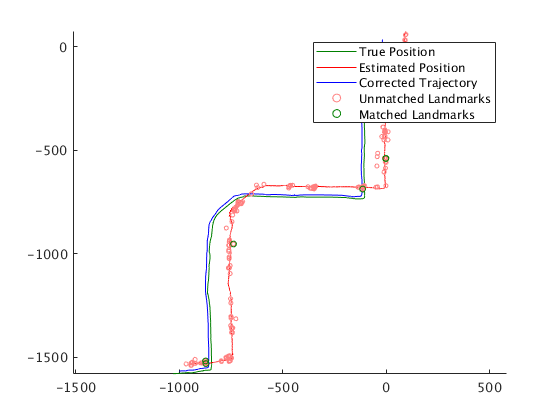
\includegraphics[width=\linewidth]{sim_results.png}
  \caption{Simulation results after observing 7 matched landmarks}
  \label{fig:simresults}
\end{figure}

\begin{figure}[thpb]
  \centering
  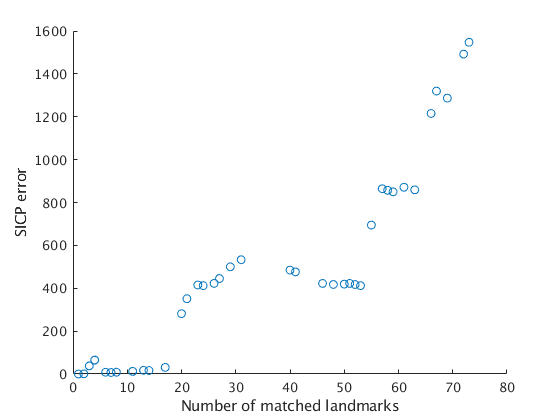
\includegraphics[width=\linewidth]{sicp_err.png}
  \caption{SICP error vs. Number of matched landmarks}
  \label{fig:sicperr}
\end{figure}

\begin{figure}[thpb]
  \centering
  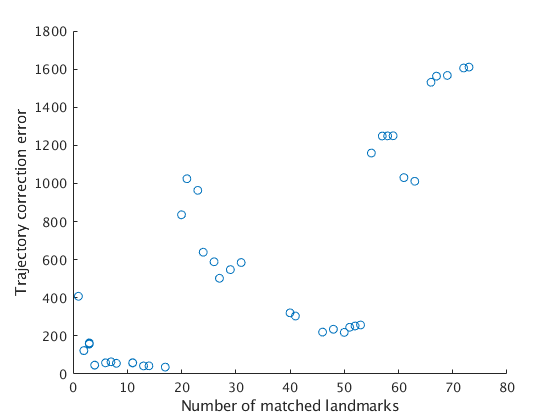
\includegraphics[width=\linewidth]{traj_err.png}
  \caption{Corrected trajectory error vs. Number of matched landmarks}
  \label{fig:trajerr}
\end{figure}

\begin{figure}[thpb]
  \centering
  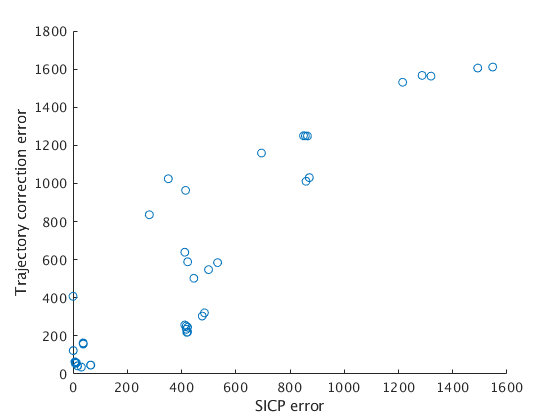
\includegraphics[width=\linewidth]{sicp_traj_err.png}
  \caption{Corrected trajectory error vs. SICP error}
  \label{fig:sicptrajerr}
\end{figure}

The data used to evaluate our method was taken from an hour long drive in downtown Chicago.
In order to test our methods ability to recover the true trajectory of the vehicle in the presence of bad GPS data, the collected GPS data was corrupted by adding an offset before passing it into the SLAM algorithm.
The GPS, odometry and landmark observation data was then replayed and passed into a MATLAB program implementing our algorithm.

In practice, many of the landmark types which were detected on the vehicle were not available in the map data. Although such landmarks can be useful in improving the trajectory estimate directly output from the SLAM algorithm, they are of no use when attempting to align the local and global maps.
As a result, a significant amount of driving time is required to obtain enough matching landmark observations in order to recover the true vehicle trajectory.

Figure \ref{fig:simresults} shows the results after finding 7 observed landmarks whose classes matched those found in the global map, which demonstrates that the true trajectory can be recovered with good accuracy.
Figure \ref{fig:sicperr} shows the error between the local map and global map after performing SICP alignment.
Figure \ref{fig:trajerr} shows the error between the corrected trajectory and the ground truth trajectory. This data shows that only a few points are necessary to recover the true trajectory. However, the dataset used had errors in some of the observed semantic classes which caused incorrect results from the SICP algorithm once those measurements were obtained.

Figure \ref{fig:sicptrajerr} shows the correlation between the SICP and corrected trajectory errors. There is a high correlation between the SICP error, which is observable without knowing the ground truth, and the error in the corrected trajectory. This indicates that the SICP error can be used as a good metric for determining whether or not the trajecory correction was successful.

\section{LIMITATIONS}

\subsection{Variable density of source and target cloud}


For the Semantic ICP algorithm the traffic signs in HERE maps are used as the target cloud. The source cloud for the Point Cloud Registration came from the drive data of mobile platform. The drive data has a high density of 450 different traffic signs in the sample drive around Chicago downtown. But the corresponding HERE HD global map have a low density of sign data and with fewer sign types. Our algorithm could find matching correspondences between 12 and 15 semantic traffic sign types, even though the drive data has hundreds of different traffic sign types. The following are some of the traffic signs with matching correspondences between source and target cloud; Pedestrian crossing warning, STOP sign, YIELD, Road Narrows Right, and Slippery When Wet.
\subsection{Mislabeled Semantics}

Sometimes, the sign types stored in the drive data are not binned perfectly. There are instances in which the traffic sign types are mislabeled or stored under different types. In our case, the sign type 46 (NO TURN ON RED sign) had many incorrect labels which resulted in wrong correspondences and caused divergence from the solution. We had to remove that specific sign type from the semantics to get the SICP to function correctly.



\section{FUTURE WORK}

\subsection{subsection placeholder}

future work placeholder


For real time implementation, we can construct a high-speed ICP algorithm by combining variants of ICP as discussed in “Efficient Variants of the ICP Algorithm” by Szymon Rusinkiewicz and Marc Levoy, Stanford University. Instead of using all the points, we can use random sampling with constant weighting and specifying a distance threshold for rejecting outlier pairs. To generate point correspondences, projection-based algorithm can be used instead of closest point method thereby reducing the wrong correlation. This algorithm can be combined with a point-to-plane error metric and the standard “select-match-minimize” ICP iteration. 


\section{HOW TO CREATE FIGURES AND TABLES REFERENCE - TO BE DELETED BEFORE SUBMISSION}
\subsection{Figures and Tables}

Positioning Figures and Tables: Place figures and tables at the top and bottom of columns. Avoid placing them in the middle of columns. Large figures and tables may span across both columns. Figure captions should be below the figures; table heads should appear above the tables. Insert figures and tables after they are cited in the text. Use the abbreviation 'Fig. 1', even at the beginning of a sentence.

\begin{table}[h]
\caption{An Example of a Table}
\label{table_example}
\begin{center}
\begin{tabular}{|c||c|}
\hline
One & Two\\
\hline
Three & Four\\
\hline
\end{tabular}
\end{center}
\end{table}


   \begin{figure}[thpb]
      \centering
      \framebox{\parbox{3in}{We suggest that you use a text box to insert a graphic (which is ideally a 300 dpi TIFF or EPS file, with all fonts embedded) because, in an document, this method is somewhat more stable than directly inserting a picture.
}}
      %\includegraphics[scale=1.0]{figurefile}
      \caption{Inductance of oscillation winding on amorphous
       magnetic core versus DC bias magnetic field}
      \label{figurelabel}
   \end{figure}
   

Figure Labels: Use 8 point Times New Roman for Figure labels. Use words rather than symbols or abbreviations when writing Figure axis labels to avoid confusing the reader. As an example, write the quantity 'Magnetization', or 'Magnetization, M', not just 'M'. If including units in the label, present them within parentheses. Do not label axes only with units. In the example, write 'Magnetization (A/m)' or 'Magnetization {A[m(1)]}', not just 'A/m'. Do not label axes with a ratio of quantities and units. For example, write 'Temperature (K)', not 'Temperature/K.'

\addtolength{\textheight}{-12cm}   % This command serves to balance the column lengths
                                  % on the last page of the document manually. It shortens
                                  % the textheight of the last page by a suitable amount.
                                  % This command does not take effect until the next page
                                  % so it should come on the page before the last. Make
                                  % sure that you do not shorten the textheight too much.

%%%%%%%%%%%%%%%%%%%%%%%%%%%%%%%%%%%%%%%%%%%%%%%%%%%%%%%%%%%%%%%%%%%%%%%%%%%%%%%%



%%%%%%%%%%%%%%%%%%%%%%%%%%%%%%%%%%%%%%%%%%%%%%%%%%%%%%%%%%%%%%%%%%%%%%%%%%%%%%%%



%%%%%%%%%%%%%%%%%%%%%%%%%%%%%%%%%%%%%%%%%%%%%%%%%%%%%%%%%%%%%%%%%%%%%%%%%%%%%%%%
\section*{APPENDIX}

Appendixes should appear before the acknowledgment.

\section*{ACKNOWLEDGMENT}

The preferred spelling of the word 'acknowledgment' in America is without an 'e' after the 'g'. Avoid the stilted expression, 'One of us (R. B. G.) thanks . . .'  Instead, try 'R. B. G. thanks'. Put sponsor acknowledgments in the unnumbered footnote on the first page.



%%%%%%%%%%%%%%%%%%%%%%%%%%%%%%%%%%%%%%%%%%%%%%%%%%%%%%%%%%%%%%%%%%%%%%%%%%%%%%%%

References are important to the reader; therefore, each citation must be complete and correct. If at all possible, references should be commonly available publications.



\begin{thebibliography}{99}

\bibitem{c1} G. O. Young, 'Synthetic structure of industrial plastics (Book style with paper title and editor),' 	in Plastics, 2nd ed. vol. 3, J. Peters, Ed.  New York: McGraw-Hill, 1964, pp. 15'64.
\bibitem{c2} W.-K. Chen, Linear Networks and Systems (Book style).	Belmont, CA: Wadsworth, 1993, pp. 123'135.
\bibitem{c3} H. Poor, An Introduction to Signal Detection and Estimation.   New York: Springer-Verlag, 1985, ch. 4.
\bibitem{c4} B. Smith, 'An approach to graphs of linear forms (Unpublished work style),' unpublished.
\bibitem{c5} E. H. Miller, 'A note on reflector arrays (Periodical style'Accepted for publication),' IEEE Trans. Antennas Propagat., to be publised.
\bibitem{c6} J. Wang, 'Fundamentals of erbium-doped fiber amplifiers arrays (Periodical style'Submitted for publication),' IEEE J. Quantum Electron., submitted for publication.
\bibitem{c7} C. J. Kaufman, Rocky Mountain Research Lab., Boulder, CO, private communication, May 1995.
\bibitem{c8} Y. Yorozu, M. Hirano, K. Oka, and Y. Tagawa, 'Electron spectroscopy studies on magneto-optical media and plastic substrate interfaces(Translation Journals style),' IEEE Transl. J. Magn.Jpn., vol. 2, Aug. 1987, pp. 740'741 [Dig. 9th Annu. Conf. Magnetics Japan, 1982, p. 301].
\bibitem{c9} M. Young, The Techincal Writers Handbook.  Mill Valley, CA: University Science, 1989.
\bibitem{c10} J. U. Duncombe, 'Infrared navigation'Part I: An assessment of feasibility (Periodical style),' IEEE Trans. Electron Devices, vol. ED-11, pp. 34'39, Jan. 1959.
\bibitem{c11} S. Chen, B. Mulgrew, and P. M. Grant, 'A clustering technique for digital communications channel equalization using radial basis function networks,' IEEE Trans. Neural Networks, vol. 4, pp. 570'578, July 1993.
\bibitem{c12} R. W. Lucky, 'Automatic equalization for digital communication,' Bell Syst. Tech. J., vol. 44, no. 4, pp. 547'588, Apr. 1965.
\bibitem{c13} S. P. Bingulac, 'On the compatibility of adaptive controllers (Published Conference Proceedings style),' in Proc. 4th Annu. Allerton Conf. Circuits and Systems Theory, New York, 1994, pp. 8'16.
\bibitem{c14} G. R. Faulhaber, 'Design of service systems with priority reservation,' in Conf. Rec. 1995 IEEE Int. Conf. Communications, pp. 3'8.
\bibitem{c15} W. D. Doyle, 'Magnetization reversal in films with biaxial anisotropy,' in 1987 Proc. INTERMAG Conf., pp. 2.2-1'2.2-6.
\bibitem{c16} G. W. Juette and L. E. Zeffanella, 'Radio noise currents n short sections on bundle conductors (Presented Conference Paper style),' presented at the IEEE Summer power Meeting, Dallas, TX, June 22'27, 1990, Paper 90 SM 690-0 PWRS.
\bibitem{c17} J. G. Kreifeldt, 'An analysis of surface-detected EMG as an amplitude-modulated noise,' presented at the 1989 Int. Conf. Medicine and Biological Engineering, Chicago, IL.
\bibitem{c18} J. Williams, 'Narrow-band analyzer (Thesis or Dissertation style),' Ph.D. dissertation, Dept. Elect. Eng., Harvard Univ., Cambridge, MA, 1993. 
\bibitem{c19} N. Kawasaki, 'Parametric study of thermal and chemical nonequilibrium nozzle flow,' M.S. thesis, Dept. Electron. Eng., Osaka Univ., Osaka, Japan, 1993.
\bibitem{c20} J. P. Wilkinson, 'Nonlinear resonant circuit devices (Patent style),' U.S. Patent 3 624 12, July 16, 1990. 
\bibitem{ref:isam} M. Kaess, 'iSAM2: Incremental Smoothing and Mapping Using the Bayes Tree,' Intl. J. of Robotics Research, 31(2), 216-235.






\end{thebibliography}




\end{document}
